
\begin{problem}
(a) Let $G = (V,E)$ be a graph with $|V| = n$, and let $k$ be an integer, where $1\le k\le n$.
Prove the following theorem:
``Suppose the the vertices in $V$ can be ordered $v_1,v_2,...,v_n$ in such a way
that each vertex $v_i$ has at most $k$ neighbors among the preceding
vertices $v_1,...,v_{i-1}$. Then $G$ can be colored with at most $k+1$ colors.''

For example, the figure below shows a graph and an ordering of its
vertices where each vertex has at most $3$ neighbors that precede it in this
ordering. So this theorem claims that this graph can be colored with $4$ colors.

	\begin{center}
	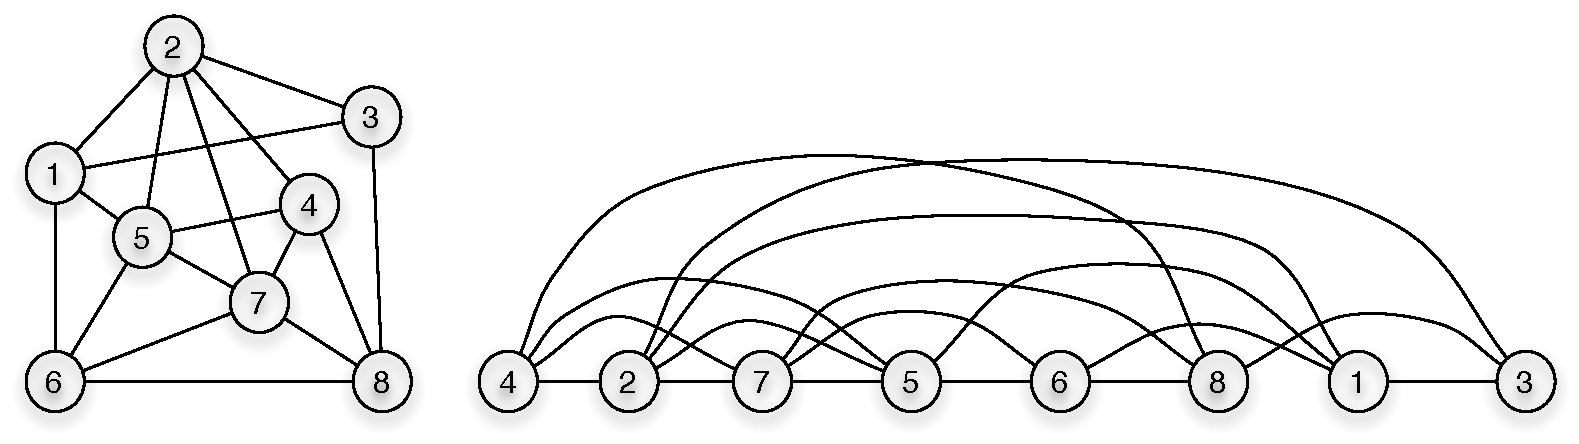
\includegraphics[width = 6in]{ordering_hw5.pdf}
	\end{center}

\noindent
(b)
Prove that the theorem in part (a) above implies the following
statement: ``If all vertices of a graph $G$ have degree at most $D$
then $G$ can be colored with at most $D+1$ colors''.
(You will cover a different proof of this theorem in the discussion. Here you
only need to show how it can be derived from part (a).)

\end{problem}

